\documentclass[preview]{standalone}
\usepackage{tikz}
\begin{document}
\thispagestyle{empty}
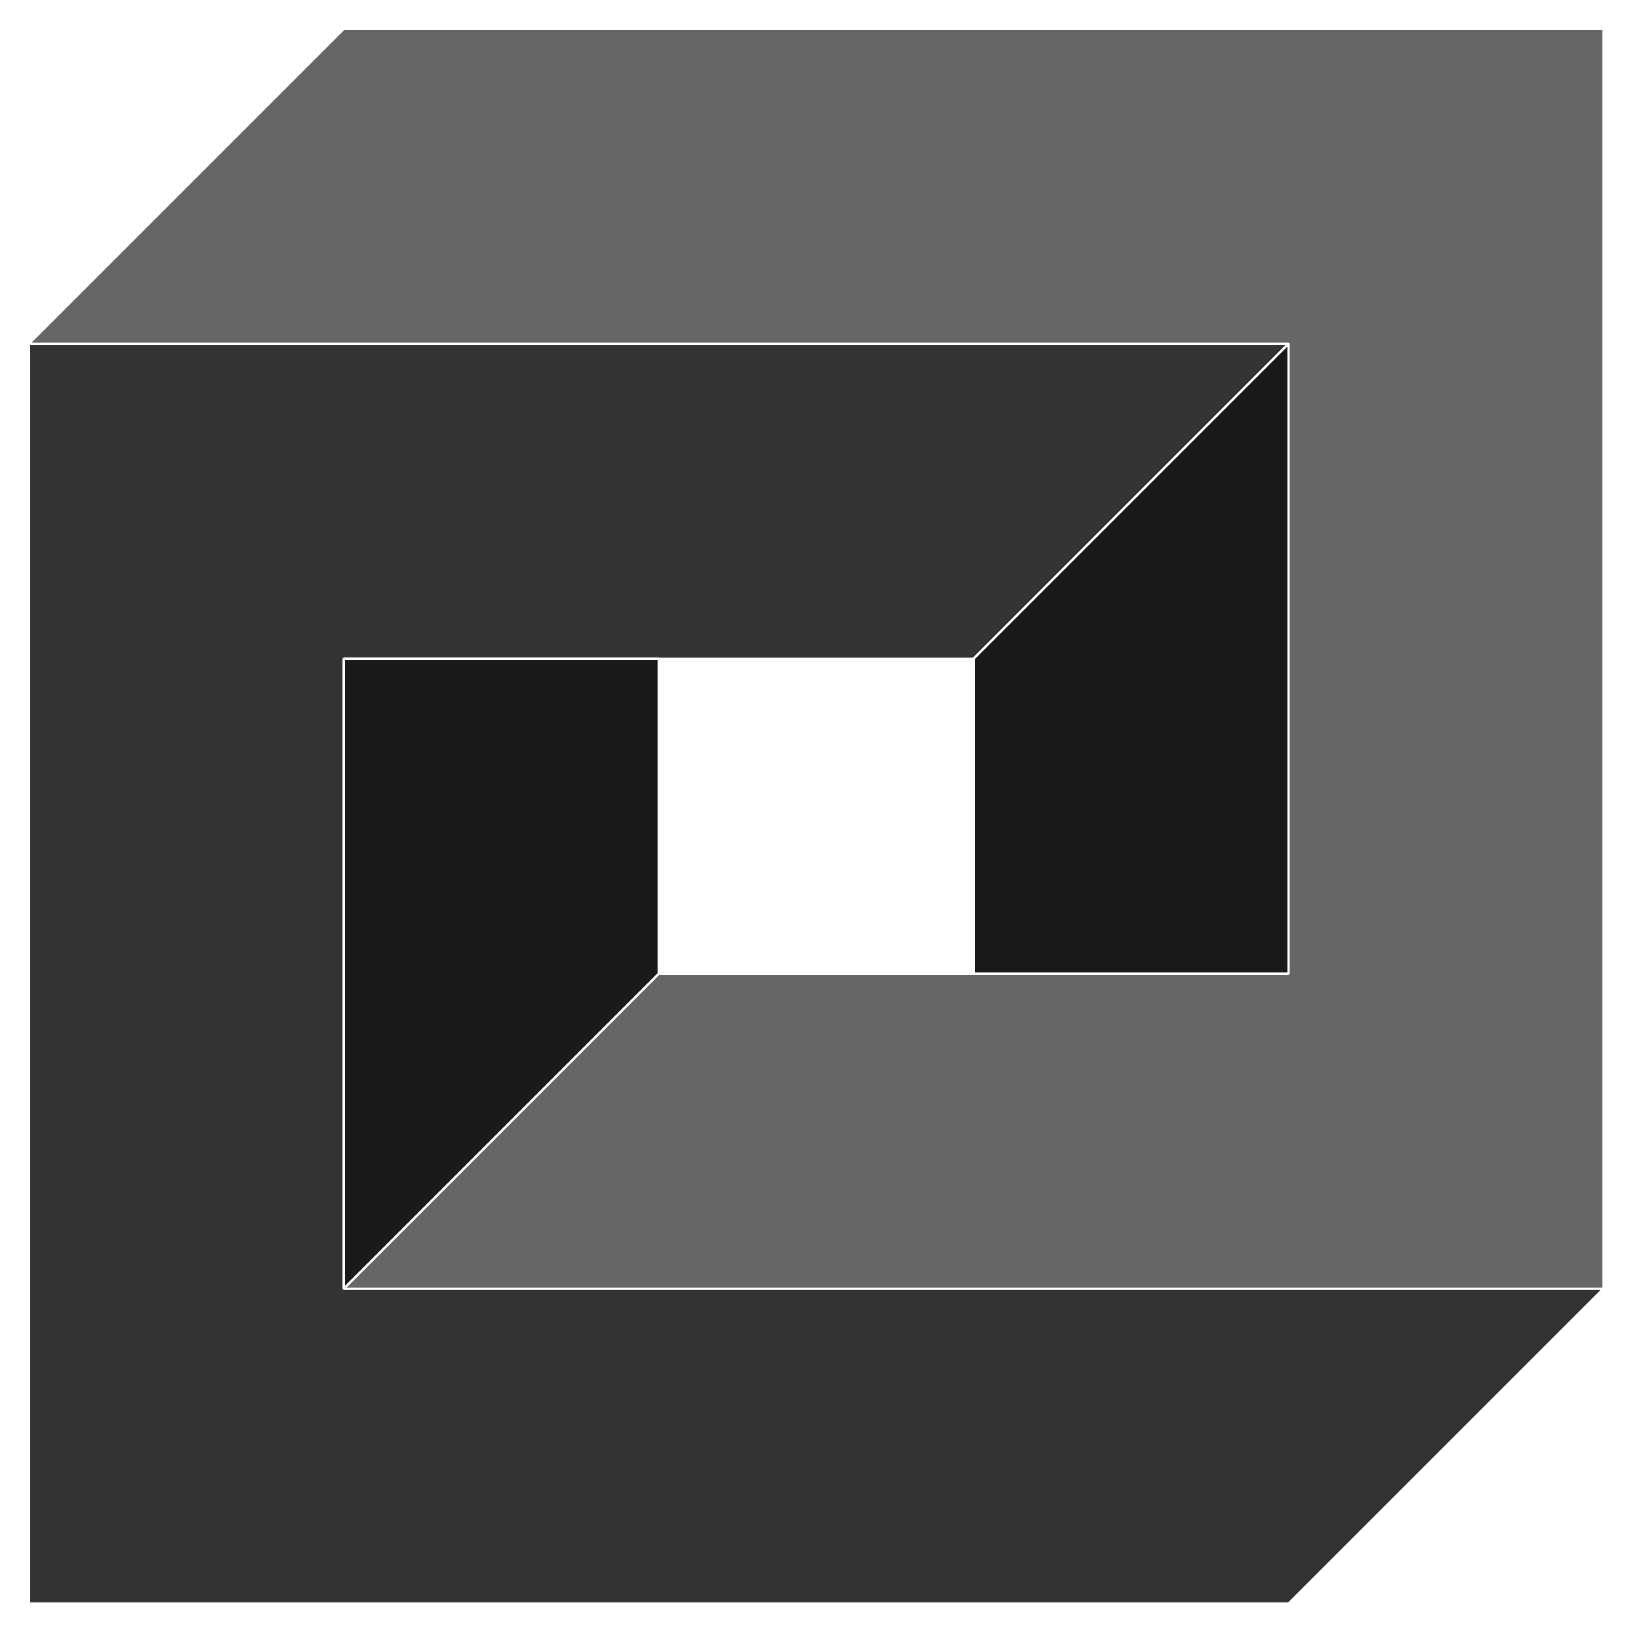
\begin{tikzpicture}[scale=1, line join=bevel]
  % \a and \b are two macros defining characteristic
  % dimensions of the impossible brick.
  \pgfmathsetmacro{\a}{4}
  \pgfmathsetmacro{\b}{16}

  \tikzset{
    apply style/.code={\tikzset{#1}},
    brick_edges/.style={thick,draw=white},
    face_colourA/.style={fill=black!80},
    face_colourB/.style={fill=black!60},
    face_colourC/.style={fill=black!90},
  }

  \foreach \theta/\v/\facestyleone/\facestyletwo in {
    0/0/{brick_edges,face_colourA}/{brick_edges,face_colourC},
    180/-\a/{brick_edges,face_colourB}/{brick_edges,face_colourC}
  }{
  \begin{scope}[rotate=\theta,shift={(\v,0)}]
    \draw[apply style/.expand once=\facestyleone]
      ({-.5*\b},{1.5*\a}) --
      ++(\b,0)            --
      ++(-\a,-\a)         --
      ++({-\b+2*\a},0)    --
      ++(0,-{2*\a})       --
      ++(\b,0)            --
      ++(-\a,-\a)         --
      ++(-\b,0)           --
      cycle;
    \draw[apply style/.expand once=\facestyletwo]
      ({.5*\b},{1.5*\a})  --
      ++(0,{-2*\a})       --
      ++(-\a,0)           --
      ++(0,\a)            --
      cycle;
    \end{scope}
  }
\end{tikzpicture}
\end{document}
